\chapter{The deployment stratagy}
\section{Introduction}
in this day and age, users expect uninterrupted access to websites around the clock.  To ensure this high level of availability, selecting the right deployment strategy is critical.  This strategy should facilitate seamless updates with minimal to no downtime for the website.  Furthermore, a robust rollback procedure should be implemented to address any unforeseen issues that may arise during deployment.  This chapter will delve into the specific deployment strategy chosen for this project, along with the rollback procedure designed to ensure a smooth recovery process in the event of failure. and the monitoring tools that will be used to monitor the web application once deployed.
\section{Sprint backlog}
\begin{longtable}[c]{
    |p{.85\textwidth}|
    p{.11\textwidth}|
    }
    \caption{Sprint 3 backlog}
    \label{tab:Sprint3_backlog}                                                                   \\
    \hline
    research the different deployment strategies and select the most appropriate one & (3 points) \\
    \hline
    research the different rollback strategies and select the most appropriate one   & (2 points) \\
    \hline
    compare the different ways to implement the deployment strategy.                 & (1 points) \\
    \hline
    implement the deployment strategy in the production release pipeline             & (2 points) \\
    \hline
    implement the rollback strategy in the production release pipeline               & (2 points) \\
    \hline
    test the downtime of the deployment during an update.                            & (2 points) \\
    \hline
    test the rollback procedure.                                                     & (1 points) \\ \hline
\end{longtable}
\section{The different deployment strategies \cite{webArticle6}}
A deployment strategy is a way to change or upgrade an application. The aim is to make the change without downtime in a way that the user barely notices the improvements.
\par Now that we know what a deployment strategy is, let's dive into the different types of deployment strategies:

\subsection*{ \textbullet\ Blue-green deployment:}
This deployment strategy involves running the new version of the software alongside the old version.
Stable or older versions of the application are always blue while newer versions are green.
When the new version has been tested and certified to meet all the requirements, the load balancer automatically switches traffic from the older version to the newer one.
\par \noindent \textbf{Advantages:} This strategy offers a quick update with simplicity and minimal impact on the users.
\par \noindent \textbf{Desadvantages:} expensive since both the new and old versions must run simultaneously.

\begin{figure}[htbp]
    \centering
    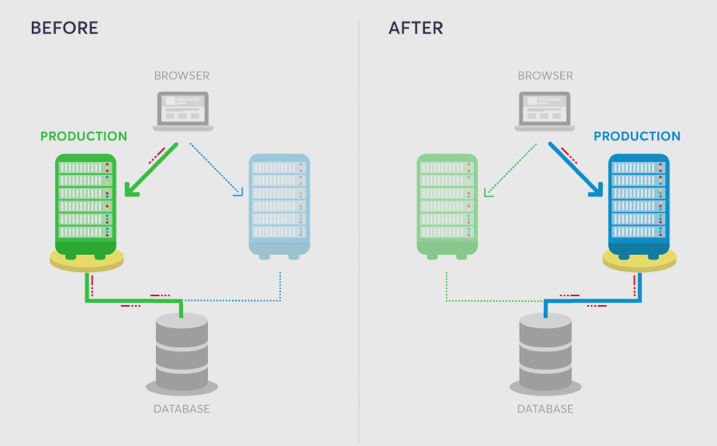
\includegraphics[width=0.9\textwidth]{blue_green_deployment.png}
    \caption{blue-green deployment strategy.}
    \label{fig:blue-green-deployment-strategy}
\end{figure}

\subsection*{ \textbullet\ Canary deployment:}
During canary deployment, the team responsible for deployment gradually redirects traffic from the older version to the new one.
This is done in small increments, allowing the team to monitor the new version's performance and quickly roll back if necessary.
\par \noindent \textbf{Advantages:} This strategy allows for better performance monitoring as well as faster and easier software rollbacks.
\par \noindent \textbf{Desadvantages:} It has a slow deployment cycle and requires more time.

\begin{figure}[htbp]
    \centering
    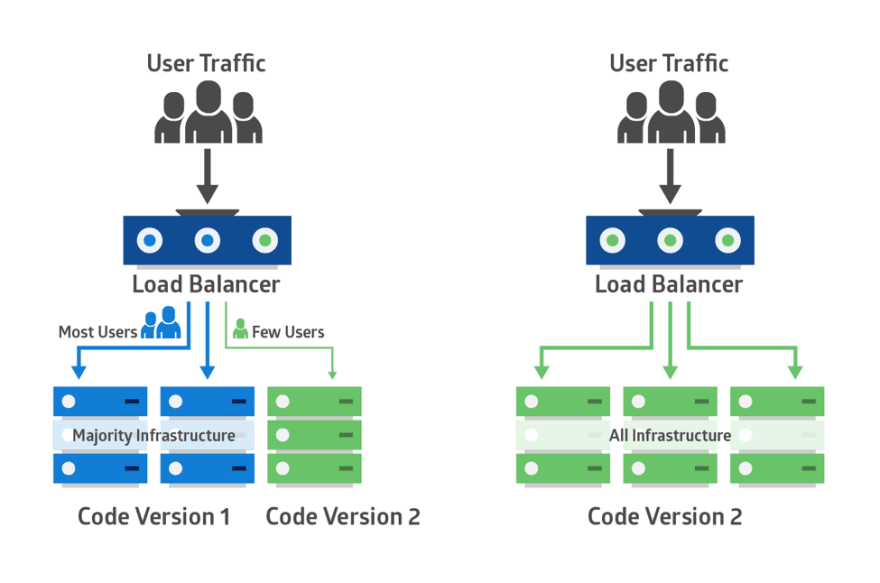
\includegraphics[width=0.8\textwidth]{canary.png}
    \caption{canary deployment strategy.}
    \label{fig:canary-deployment-strategy}
\end{figure}

\subsection*{ \textbullet\ Ramped/Rolling deployment:}
The ramped deployment strategy gradually changes the older version to the new version. Unlike canary deployment, the ramped deployment strategy replaces instances of the old application version with instances of the new application version one instance at a time.
\par \noindent \textbf{Advantages:} This strategy costs less than canary and blue-green deployment strategies since every instance not used is destroyed.
\par \noindent \textbf{Desadvantages:} In case of an unexpected event, the rollback process takes longer than the other strategies.

\subsection*{ \textbullet\ A/B testing:}
Developers deploy the new version alongside the older version in A/B testing deployment. However, this new version is only available to a limited number of users, who are selected according to certain conditions and parameters. Location, device type, UI language, and operating system can serve as parameters for selecting these users.
\par \noindent \textbf{Advantages:} The use of real-time statistical data can help developers make informed decisions about their software.
\par \noindent \textbf{Desadvantages:} This strategy is complex and requires a high-end load balancer that can access the application layer.

\subsection*{ \textbullet\ Verdict}
Given our need for swift deployments and near-instant rollbacks, coupled with a cost-effective and manageable infrastructure, a blue-green deployment strategy is the ideal choice.

\section{The different ways to implement the deployment strategy}
\subsection*{ \textbullet\ Utilizing Infrastructure as Code (IaC) and Traffic Management}
this method needs these steps to be implemented in the pipeline:
\begin{itemize}
    \item Create a green environment using IaC tools.
    \item deploy the new version of the application to the green environment.
    \item Use the traffic management resource to switch the traffic from the blue environment to the green environment.
\end{itemize}
\textbf{Advantages:} This method is cost-effective and more customizable(because you can choose any SKU for the requirements).
\\
\textbf{Desadvantages:} It takes longer during updates since we need to create an environment each time. Also, it adds the complexity of adding a load balancer to the infrastructure.
\subsection*{ \textbullet\ Leveraging Azure App Service Deployment Slots}
Deployment slots are live apps with their host names. App content and configuration elements can be swapped between two deployment slots, including the production slot.
\begin{itemize}
    \item Create a deployment slot for the new version of the application.
    \item Deploy the new version of the application to the deployment slot.
    \item Swap the deployment slot with the production slot.
\end{itemize}
\textbf{Advantages:} It is way simpler to implement than the first method, and it is faster during updates.
\\
\textbf{Desadvantages:} This method requires at least the Standard SKU for the App Service Plan.
\subsection*{ \textbullet\ Verdict:}
since this strategy is implemented in the production environment choosing the Strandard SKU is acceptable. So to avoid unnecessary complexity and to speed up the deployment process, we will use the Azure App Service Deployment Slots method.
\\

\begin{figure}[htbp]
    \centering
    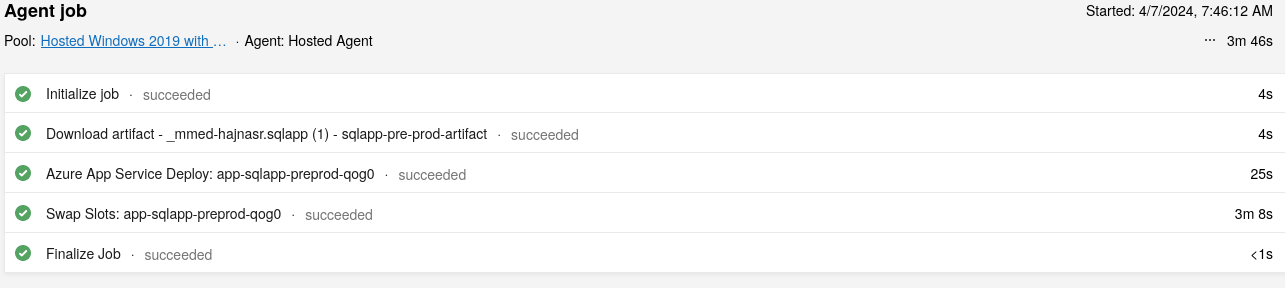
\includegraphics[width=0.9\textwidth]{blue-green_implemented.png}
    \caption{Azure App Service Deployment Slots implementation.}
    \label{fig:deployment-slots}
\end{figure}

\begin{figure}[htbp]
    \centering
    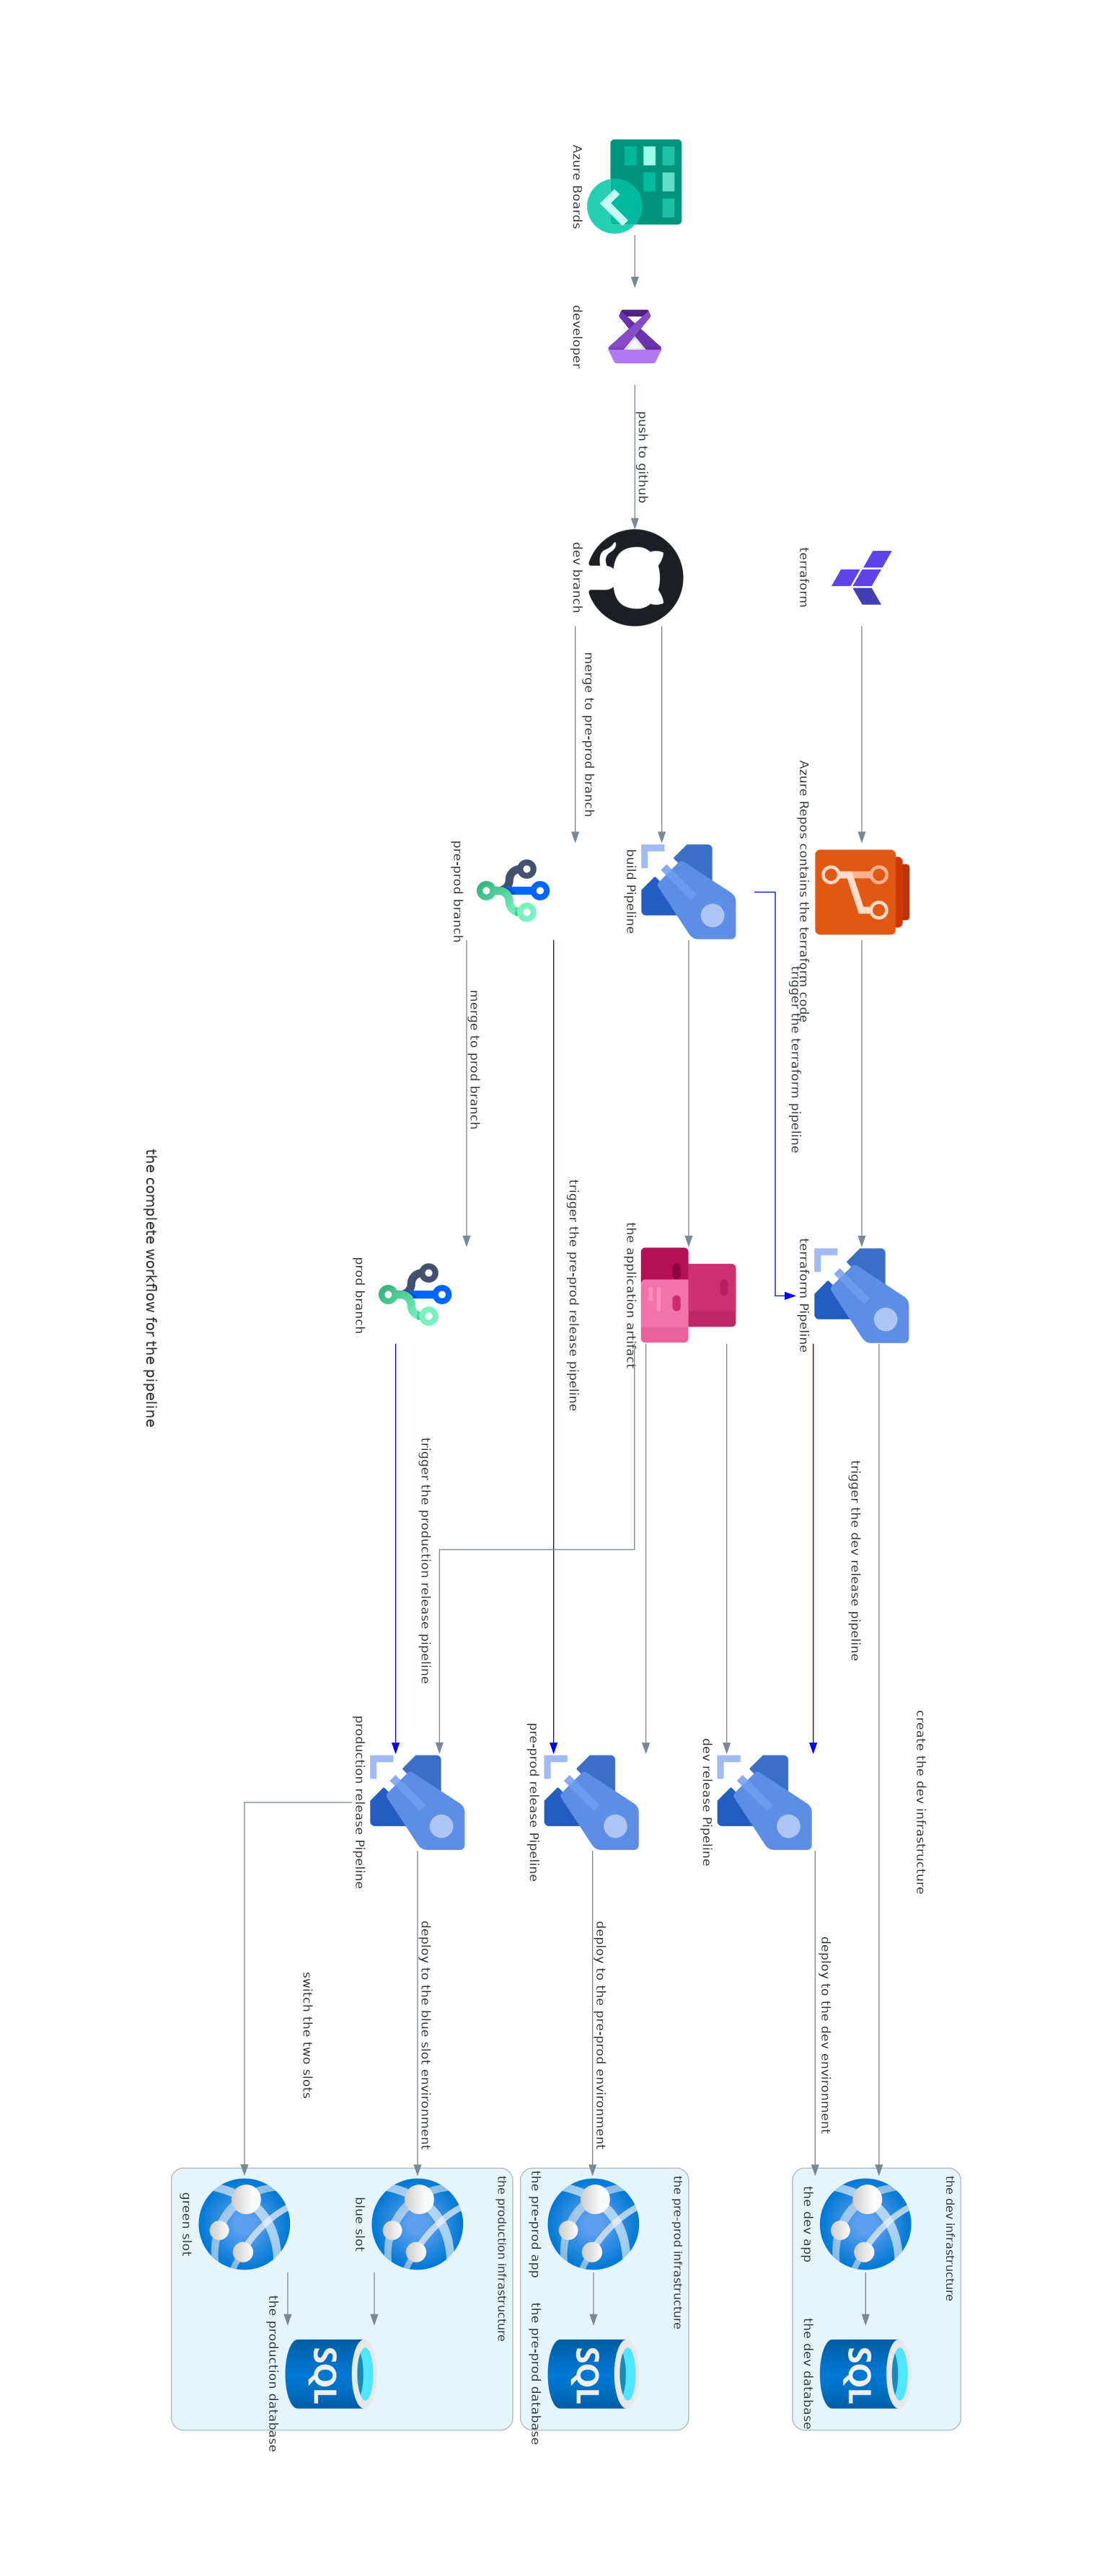
\includegraphics[width=0.6\textwidth]{full_workflow.png}
    \caption{the full workflow of the deployment strategy.}
    \label{fig:deployment-strategy-full-workflow}
\end{figure}

\pagebreak
\section{The rollback strategy}
the deployment pipeline incorporates a robust rollback strategy to ensure minimal disruption and user satisfaction.
\subsection*{ \textbullet\ Deployment process}

\begin{itemize}
    \item \textbf{New Version Deployment:} The new version is deployed through the pipeline.
    \item \textbf{Automatic Rollback on Deployment Failure:} Any errors encountered during deployment will trigger an automatic rollback. This ensures the system quickly reverts to the previous stable version, minimizing downtime and potential data loss.
    \item \textbf{User Feedback and Rollback Option:} Users have the opportunity to provide feedback on the new version. If a significant number of users express dissatisfaction, an admin can initiate a rollback.
\end{itemize}

\subsection{The rollback retention}
\textbf{30-Day Rollback Window:}
The pipeline, including the rollback option, remains accessible for 30 days after deployment. This window provides ample time for user feedback and admin decision-making.
\\ \noindent
\textbf{Automatic Rollback Rejection After 30 Days:}
If no rollback is initiated within 30 days, the rollback stage is automatically deactivated. This prevents holding onto outdated rollback options indefinitely and we can delete the old version slots to avoid extra costs.
\\
\begin{figure}[htbp]
    \centering
    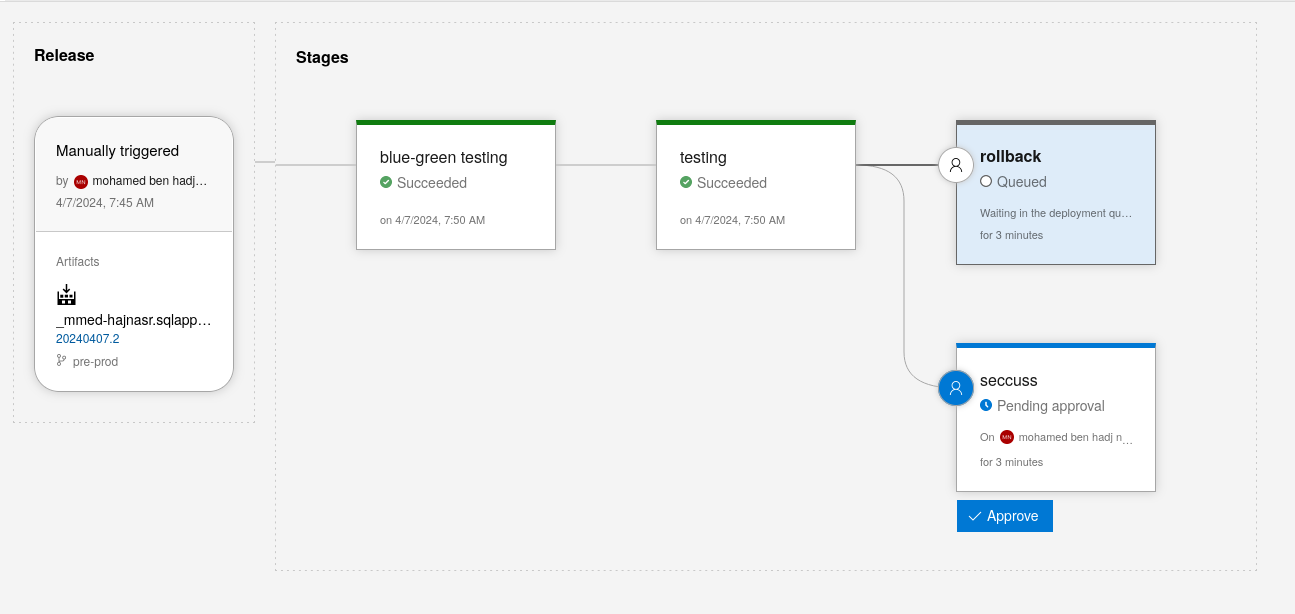
\includegraphics[width=0.9\textwidth]{choice.png}
    \caption{the rollback strategy implementation}
    \label{fig:rollback-strategy}
\end{figure}

\begin{figure}[htbp]
    \centering
    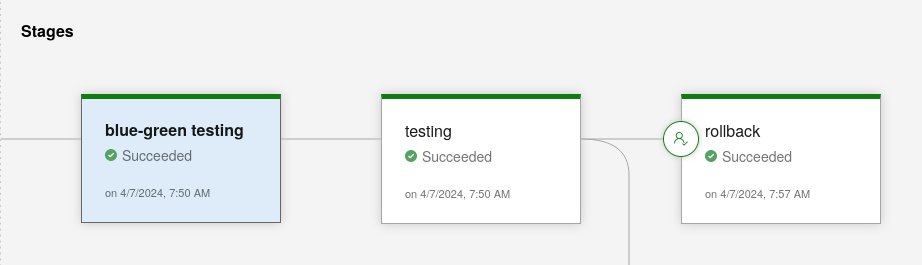
\includegraphics[width=0.9\textwidth]{rollback.png}
    \caption{seccuss rollback}
    \label{fig:rollback-seccuss}
\end{figure}

\section{The monitoring strategy \cite{webArticle7}}
we will use different monitoring tools offered by Azure to monitor the web application once deployed.
\begin{itemize}
    \item \textbf{Azure Health check:} This tool will monitor the health of the web application and notify the admin if any issues arise.
    \item \textbf{Insights:} Application Insights monitors the availability, performance, and usage of your web applications, so you can identify and diagnose errors without waiting for a user to report them.

          \begin{figure}[htbp]
              \centering
              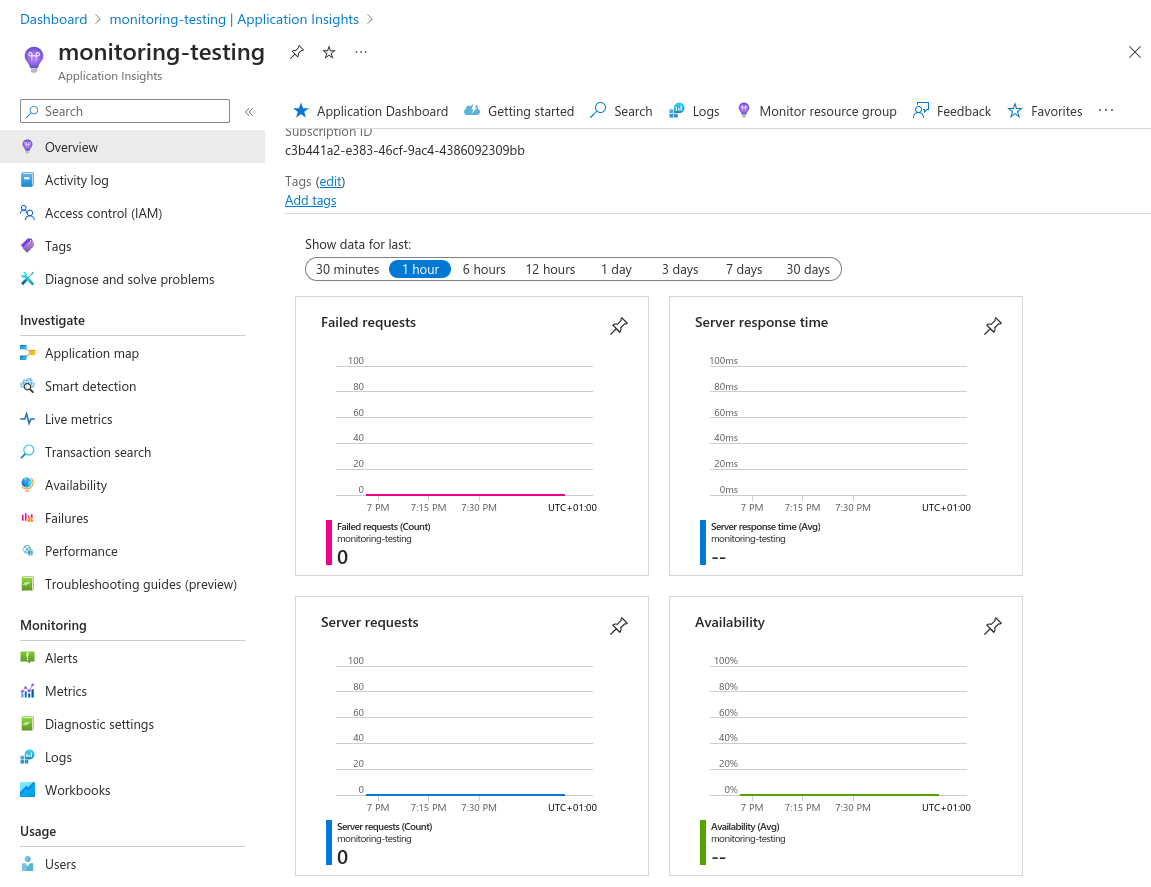
\includegraphics[width=0.7\textwidth]{monitoring-insights.png}
              \caption{monitoring insights set up}
              \label{fig:monitoring-insights}
          \end{figure}

    \item \textbf{Alerts:} Alerts can be set up to notify the admin of any issues that arise with the web application. unlike Health check, this option is highly customizable.

          \begin{figure}[htbp]
              \centering
              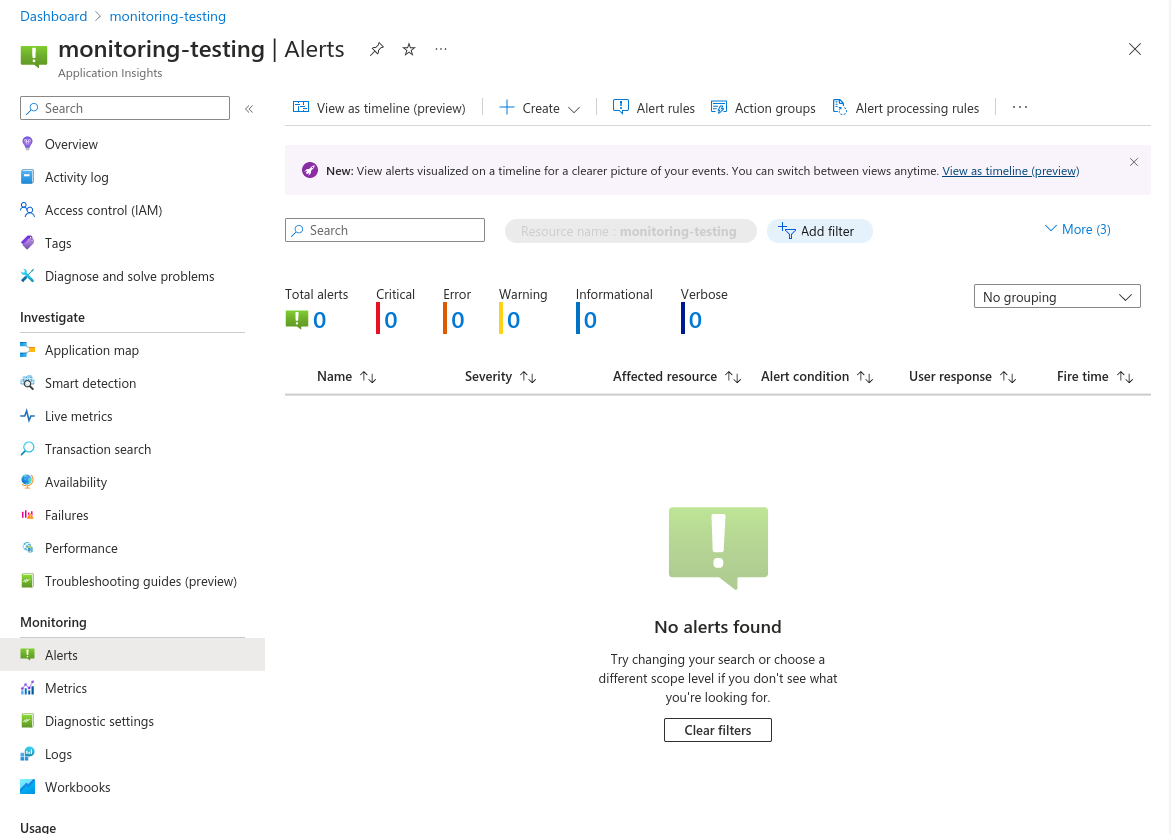
\includegraphics[width=0.7\textwidth]{alert-dashboard.png}
              \caption{in this dashboard, you can check the status of the alerts.}
              \label{fig:monitoring-alerts}
          \end{figure}

          \begin{figure}[htbp]
              \centering
              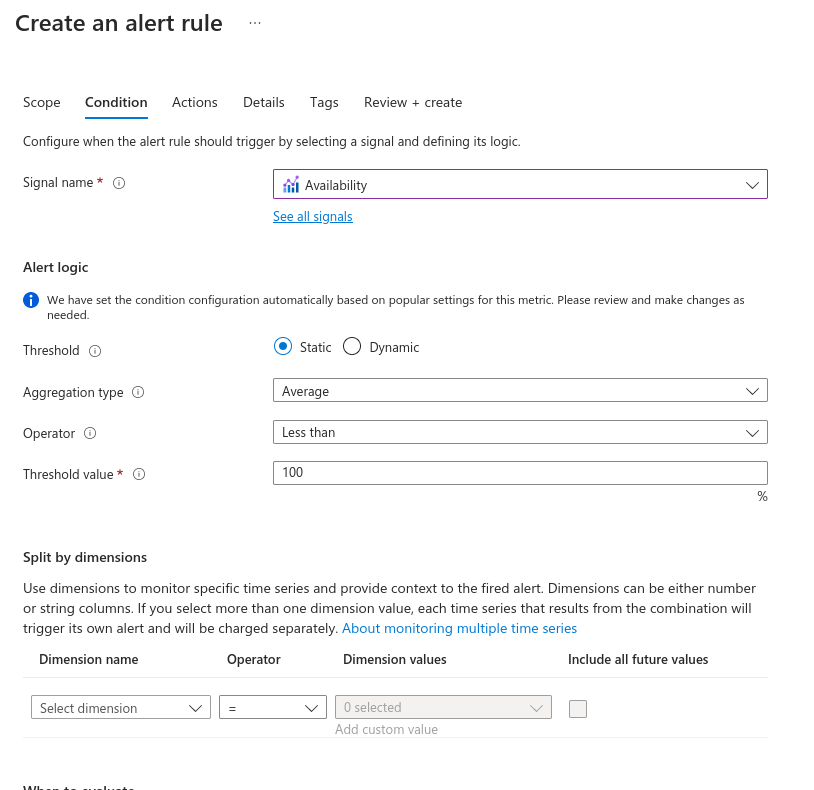
\includegraphics[width=0.5\textwidth]{alert-rule.png}
              \caption{here you can set up the alerts.}
              \label{fig:monitoring-set-up-alerts}
          \end{figure}

    \item \textbf{Metrics:} Metrics provide a detailed view of the web application's performance, including response time, request rate, and error rate.

          \begin{figure}[htbp]
              \centering
              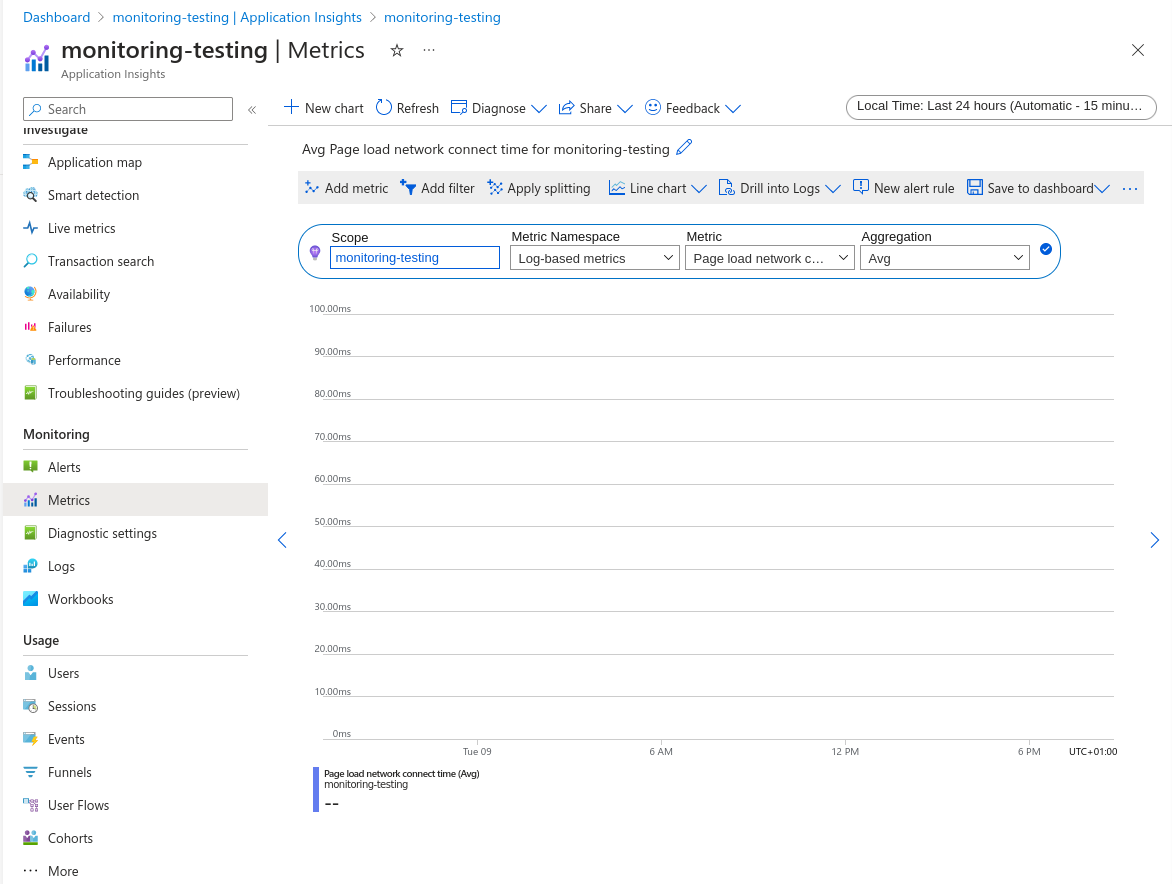
\includegraphics[width=0.8\textwidth]{metrics.png}
              \caption{metrics dashboard}
              \label{fig:monitoring-metrics}
          \end{figure}

    \item \textbf{Log Analytics:} Log Analytics provides a centralized location for monitoring and analyzing the web application's logs. This tool can help identify issues and troubleshoot problems quickly.

          \begin{figure}[htbp]
              \centering
              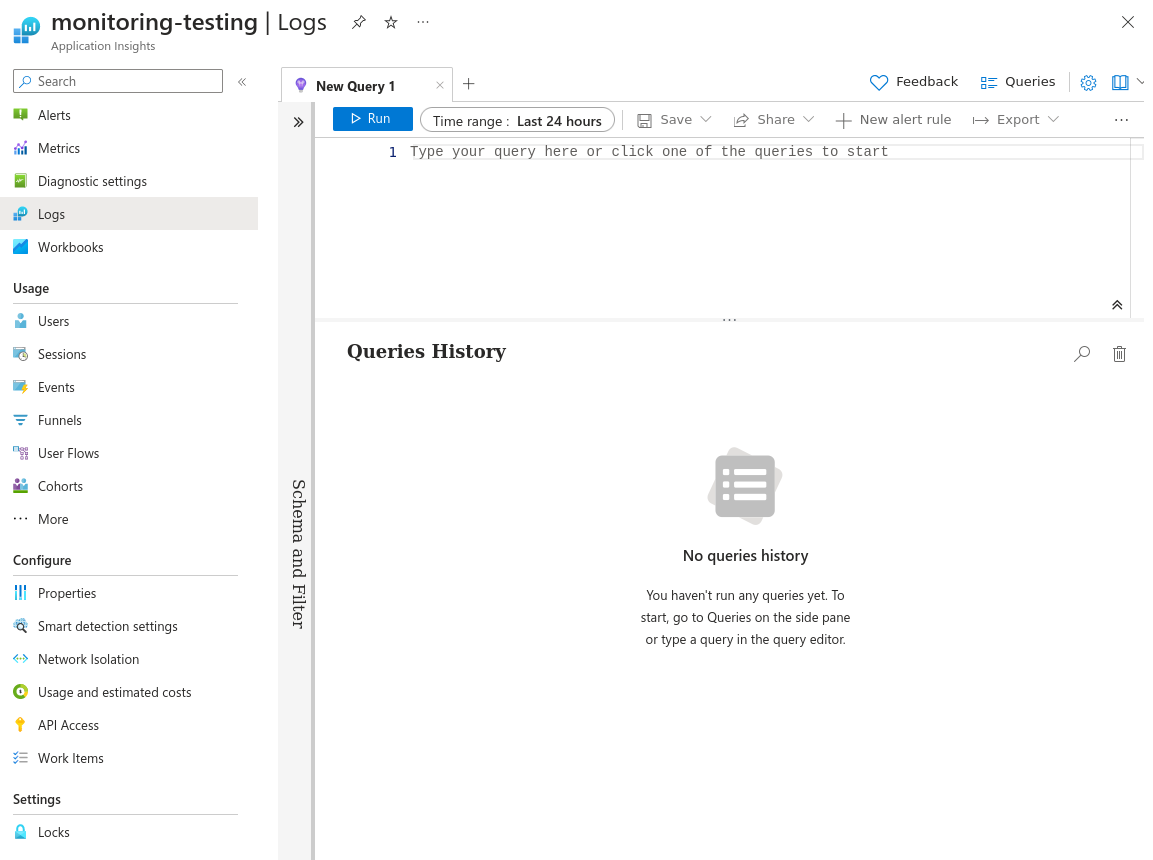
\includegraphics[width=0.8\textwidth]{query-logs.png}
              \caption{log analytics dashboard}
              \label{fig:monitoring-log-analytics}
          \end{figure}

\end{itemize}
\pagebreak
\section*{Conclusion}
In conclusion, this chapter has outlined the deployment strategy chosen for this project, which is a blue-green deployment strategy. This strategy was selected due to its ability to provide swift deployments with minimal downtime and near-instant rollbacks. Additionally, a rollback strategy has been implemented to ensure a smooth recovery process in the event of any unforeseen issues during deployment. The rollback strategy includes a 30-day rollback window to allow for user feedback and admin decision-making. Finally, a monitoring strategy has been established to monitor the health, performance, and usage of the web application once deployed. This monitoring strategy utilizes various Azure monitoring tools, including Application Insights, Health Checks, Alerts, Metrics, and Log Analytics. By implementing these strategies, we can ensure a smooth and successful deployment process for our website.
